\chapter{Supplementary materials for \autoref{chap:CMZ}}

\subsection{Normal and LogNormal models of population data}
\label{ssec:NormalModels}

We first investigated the appropriateness of Normal vs. LogNormal models for measured and calculated parameters of the CMZ and the neural retina, presented in \autoref{PLHRtable}.

\begin{table}[!ht]
    \centering
    \caption{
    {\bf Likelihood ratio comparison between Normal and Log-Normal models of retinal population parameters}}
    \begin{tabular}{|l|l|l|l|}
    \hline
    {\bf Parameter} & {\bf $\mathcal{N}$ logLH} & {\bf Log-$\mathcal{N}$ logLH} & {\bf logLR} \\ \hline
    Sectional PCNA+ve & -285.611 & {\bf -283.214} & 2.397\\ \hline
    Lens diameter & {\bf -203.102} & -203.854 & -0.752\\ \hline
    CMZ annular pop.($\dagger$)  & -484.768 & {\bf -482.733} & 2.035\\ \hline
    RPE length & {\bf -368.232} & -368.609 & -0.377\\ \hline
    CR thickness ($\dagger$) & {\bf -240.858} & -241.032 & -0.174\\ \hline
    CR volume ($\dagger$) & -1091.615 & {\bf -1091.146} & 0.469\\ \hline
    \end{tabular}
    \begin{flushleft} $\mathcal{N}$: Normal distribution. logLH: logarithm of p(D|M), the likelihood of the data given the model. logLR: logarithm of the likelihood ratio; positive ratios in favour of the log-$\mathcal{N}$ model. Largest likelihoods are bolded. $\dagger$: Calculated quantities. Sectional PCNA+ve: population of PCNA-positive CMZ RPCs per 14$\mu$m cryosection. CMZ annular pop: population of annular CMZ. RPE: retinal pigmented epithelium. CR: cellular retina.
    Methods in \autoref{ssec:PCNA} and \autoref{ssec:CMZretmeas}.
    Code in \autoref{ssec:a10popsurvey}.
    \end{flushleft}
    \label{PLHRtable}
\end{table}

These results suggest that the organism-level population distribution of eye-level CMZ population counts, as assayed by PCNA immunostaining, is better modelled Log-Normally than Normally. This is true whether we test the primary per-section count meaurements, or the estimated whole-annulus population, even though this quantity is calculated using the Normally-distributed lens diameter\footnote{The apparent superiority of the Normal model for lens diameter may be due to the paucity of data at later time points; as described in \autoref{ssec:CMZretmeas}, lenses are difficult to retain in this histological context.}. The most likely Log-Normal representations of the CMZ populations are about two orders of magnitude more likely than the Normal alternative. Additionally, although Normal models are slightly favoured for describing the population-level distributions of RPE length and cellular retina thickness, the derived cellular retina volume quantity is better modeled by a Log-Normal distribution. 

Since the choice of model describing the estimated annular population and retinal volume is critical to the success of later inferences, we used Galilean Monte Carlo-Nested Sampling (GMC-NS) to estimate the Bayesian evidence (the marginal probability of the data over all model parameterisations) for these hypotheses. Evidence estimates and ratios are presented in Table \ref{PZRtable}.

\begin{table}[!ht]
    \centering
    \caption{
    {\bf Evidence favours Log-Normal models of retinal population parameters}}
    \begin{tabular}{|l|l|l|l|l|}
    \hline
    {\bf Parameter} & {\bf $\mathcal{N}$ logZ} & {\bf Log-$\mathcal{N}$ logZ} & {\bf logZR} & {\bf $\sigma$ significance}\\ \hline
    CMZ Population & -1457.0 ± 3.7 & {\bf -1005.0 ± 3.5} & 452.1 ± 5.1 & 89.45479335402516\\ \hline
    Estimated Retinal Volume & -2042.2 ± 3.3 & {\bf -1525.2 ± 4.1} & 517.0 ± 5.3 & 97.87822790648408\\ \hline
    \end{tabular}
    \begin{flushleft} $\mathcal{N}$: Normal distribution. logZ: logarithm of p(D), the marginal likelihood of the data, or model evidence. logZR: evidence ratio; positive ratios in favour of the log-$\mathcal{N}$ model. Largest evidence values bolded. CR: cellular retina.
        Methods in \autoref{ssec:CMZpopvolest}.
        Code in \autoref{ssec:a10nvln}.
    \end{flushleft}
    \label{PZRtable}
\end{table}

Full estimation of the Bayesian evidence for the Normal vs. Log-Normal hypotheses for our calculated parameters produces confirms the rough calculation of likelihood ratio from the single-fit MAP models, although the extent to which LogNormal models are better justified than Normal differs between the methods.

If between-individual variation in retinal CMZ population and retinal volume are both well-modelled Log-Normally, the question of their independence arises. It seems plausible that the size of the CMZ population would be roughly proportional to the overall volume of the retina, after postembryonic central specification, and establishment of the peripheral CMZ remnant. Moreover, since the growth of retinal volume over the life of the organism is driven primarily by the CMZ\footnote{One observes occasional proliferative clusters in the central retina throughout the life of the fish; these are typically ascribed to M\"{u}ller glial repair processes. I am unaware of any estimate as to the relative contribution of these clusters vs. the CMZ. As we shall see, there is probably more turnover in the specified retina than previously believed. As a result, the relative contribution of these central clusters should probably be subject to statistical estimation; they may be more significant than mere lesion-repair sites.}, it seems likely that this volume is well correlated with the size of the CMZ. Since the manner in which we model the CMZ differ depending on our assessment of the dependence of these retinal parameters, we performed Bayesian model selection by the \hyperref[ssec:EmpiricalBayes]{Empirical Bayes} method for linear regression, which provides for direct estimation of the evidence for models consisting of linear equations of variables \cite{Bishop2006}.

We find that individual CMZ population and retinal volume estimates are best described by uncorrelated models at in all ages, with the exception of 23.0 dpf, where the evidence weakly favours correlation. It is interesting that the evidence in favour of non-correlation is weakest between 17 and 30 dpf, suggesting the correlation at 23.0 dpf is not spurious, but is related to CMZ activity at this time. These data are displayed in \autoref{corrtable}. Of particular importance are the data for 3dpf embryos, as we intend to seed model retinae with CMZ populations and volumes drawn from these distributions. The data for these animals are plotted in \autoref{gausscorrelation}. The general lack of correlation between CMZ population and retinal volume estimates may be due to the loss of information involved in the estimation calculations; on the other hand, it is more plausible that CMZ population should be associated with the rate of retinal volume growth rather than the volume of the retina itself, which suggests that the rate of retinal contribution from the CMZ is probably highest between 17 and 23 days. Because growth rate data are unavailable for single individuals, we cannot make this inference directly.

\begin{table}[!ht]
    \centering
    \caption{{\bf Evidence favours uncorrelated linear models of CMZ-population and retinal volume over time}}
    \begin{tabular}{|l|l|l|l|}
        \hline
        {\bf Age (dpf)} & {\bf Uncorrelated logZ} & {\bf Correlated logZ} & {\bf logZR}\\ \hline
        3.0 & {\bf -87.651} & -91.902 & 4.252\\ \hline
        5.0 & {\bf -90.0} & -92.362 & 2.362\\ \hline
        8.0 & {\bf -90.918} & -96.013 & 5.095\\ \hline
        12.0 & {\bf -91.183} & -99.049 & 7.866\\ \hline
        17.0 & {\bf -94.818} & -96.668 & 1.85\\ \hline
        23.0 & -103.386 & {\bf -103.219} & 0.167\\ \hline
        30.0 & {\bf -103.511} & -104.092 & 0.581\\ \hline
        60.0 & {\bf -115.025} & -118.169 & 3.144\\ \hline
        90.0 & {\bf -113.533} & -122.427 & 8.894\\ \hline
        180.0 & {\bf -116.778} & -124.547 & 7.769\\ \hline
        360.0 & {\bf -121.016} & -128.637 & 7.621\\ \hline
        \end{tabular}
    \begin{flushleft} logZ: logarithm of p(D), the marginal likelihood of the data, or model evidence. logZR: evidence ratio; positive ratios in favour of the uncorrelated model. Largest evidence values bolded.
    Methods in \autoref{ssec:CMZpopvolest}, \autoref{ssec:CMZEmpBayes}.
    Code in \autoref{ssec:a10correlation}.
    
    \end{flushleft}
    \label{corrtable}
\end{table}

\begin{figure}[!h]
    \makebox[\textwidth][c]{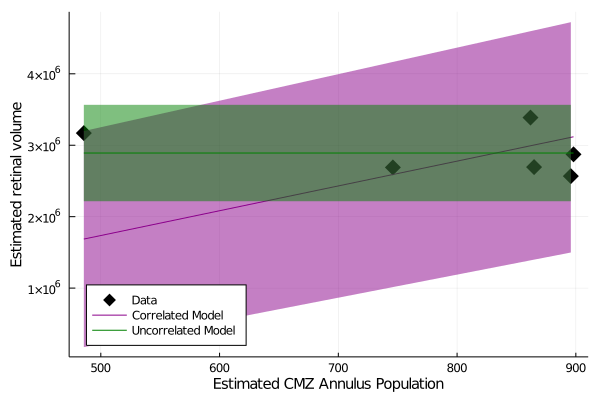
\includegraphics[width=.75\textwidth]{cmz/3dcorr.png}}    
    \caption{{\bf CMZ population and retinal volume estimates are uncorrelated at 3dpf}}
    Individual CMZ population estimate vs retinal volume estimate for 3dpf animals. Uncorrelated and correlated linear models of these variables are plotted as the mean$\pm$95\% CI of the predictive distribution of the fitted model. 
    Methods in \autoref{ssec:CMZpopvolest}, \autoref{ssec:CMZEmpBayes}.
    Code in \autoref{ssec:a10correlation}.
    \label{gausscorrelation}
\end{figure}

\section{Materials and methods}
\subsection{Zebrafish husbandry}
Zebrafish husbandry was performed as described in \autoref{ssec:husbandry}.
\subsection{PCNA Immunohistochemistry}
Anti-PCNA immunohistochemistry was performed as described in \autoref{ssec:PCNA}.
\subsection{Thymidine analogue histochemistry}
\label{ssec:CMZEdU}
Both cumulative thymidine analogue histochemistry presented in \autoref{ssec:CMZcumedu}, as well as the pulse-chase histochemistry used for the study of neural fate in \autoref{sec:neuralfate} were performed by the methods described in \autoref{ssec:SMMEcumedu} and \autoref{ssec:SMMEwholeretina}, respectively, except that the data from the whole retinal labelling experiment derives from 14\si{micro}{metre} transverse and coronal cryosections (n=3-6 animals per axis, per age). 

\subsection{Lineage tracing immunohistochemistry}
\label{ssec:CMZlintrace}
Embryos from wild-type AB crosses (staining groups 2 and 3) and \textit{Tg(Isl2b:GFP)} crosses (staining group 1). The \textit{Tg(Isl2b:GFP)} line was the kind gift of the late Dr. Chi-Bin Chien. Embryos were collected and reared as described in \autoref{ssec:husbandry}. Embryos were divided into three groups, to be pulsed with EdU at 3, 23, and 90 dpf and sacrificed after a 7 day chase period. In 3 and 23dpf larvae, animals were pulsed by allowing them to swim freely in a 10mM EdU solution for 2 hours. In 90dpf animals, 10\si{micro}{liters} of 10mM EdU was injected intraperitoneally. After 7 days, animals were sacrificed and coronal cryosections were obtained as described in \autoref{ssec:PCNA}. These cryosections were divided into staining groups according to their genetic origin, as mentioned above.

Cryosections from all staining groups were allowed to dry briefly at room temperature (RT), before rehydration in PBS for 30 minutes at RT.  Subsequently, sections were blocked in 0.2\% Triton X-100 + 2\% goat serum in PBS for 30 minutes at RT. Primary antibody incubations were as follows for each numbered staining group:

\begin{enumerate}
    \item Covance rabbit anti-Pax6 primary antibody diluted 1:200 in blocking solution incubated at 4\degree C overnight.
    \item Chemicon mouse anti-GS primary antibody diluted 1:500 in blocking solution at 4\degree C overnight.
    \item ZIRC mouse anti-Zpr1 primary antibody diluted 1:400 in blocking solution at 4\degree C overnight.
\end{enumerate}

After these overnight incubations, primary antibodies were removed and all sections were rinsed five times in PDT (PBS + 1\% DMSO + 0.1\% Tween-20). Secondary antibody incubations were as follows for each numbered staining group:

\begin{enumerate}
    \item Goat anti-rabbit Cy3-conjugated 2º antibody diluted 1:100 in blocking solution at 37°C for 2 hr.
    \item Goat anti-mouse Cy2-conjugated 2º antibody diluted 1:100 in blocking solution at 37°C for 2 hr.
    \item Goat anti-mouse Cy2-conjugated 2º antibody diluted 1:100 in blocking solution at 37°C for 2 hr.
\end{enumerate}

Staining group 2 was subsequently incubated with Santa Cruz rabbit anti-PKC$\beta$ 1º antibody diluted 1:100 in blocking solution at 4°C overnight. The next day, this second primary antibody was removed, and the group sections were rinsed in PDT as above. A further goat anti-mouse Cy2-conjugated 2º antibody diluted 1:100 in blocking sol’n was applied at 37°C for 2 hr.

After each staining group's final secondary antibody was removed, slides were rinsed 3x in PDT, then stained for EdU with an Alexa 647 azide. After another three PDT rinses, 100 ug/mL Hoechst 33258 was applied for 15 minutes at RT. Five PDT rinses, after which all slides were mounted, slipped, and sealed.

\subsection{4C4 immunohistochemistry}
\label{ssec:CMZ4C4histo}
The 4C4 antibody was a generous gift of Dr. Pamela Raymond. It has been empirically determined to mark microglia \cite{Becker2001}. It was used according to the methods described above with a Cy2 secondary antibody.

\subsection{Confocal micrograph acquisition and processing}
All confocal micrographs presented in \autoref{chap:CMZ} were acquired on a Leica TCS SP5 II microscope, operated using the LAS AF microscopy software (Leica). Data was assessed by using Bitplane Imaris software (v1.5.1). Specifically, the Imaris watershed segmentation algorithm was applied to the nuclear counterstain channel to segment cellular nuclei. Colocalisation of particular markers (ie. PCNA, EdU, or lineage markers) was assessed by thresholding signal from these channels with the segmented nuclear volumes to produce a subpopulation of colabelled nuclei. The segmented Imaris scenes and the associated settings are available in the thesis \hyperref[sec:archive]{HDD archive}.

\subsection{Retinal measurements}
\label{ssec:CMZretmeas}
The developmental morphology study presented in \autoref{morphology} was conducted by using the LAS AF software measurement tools on transmitted light data collected in the process of conducting the confocal survey presented in \autoref{CMZoverall}. Each measurement point is, therefore, likewise the average of the value three central coronal cryosections. Retinal thickness was the linear thickness of the entire cellular retina and its plexiform layers at the center of the section, and the layer thicknesses reflect segments along this line, with the addition of RPE thickness. RPE length was measured in approximating segments from the dorsal to the ventral extrema. Lens diameter was measured in any sections which retained the lens; this was rare at older ages, when the lens sections tend to separate readily as soon as the cryosection is rehydrated. Optic nerve diameter was measured at its thickest point.

\subsection{Estimation of overall CMZ population and retinal volume}
\label{ssec:CMZpopvolest}
The overall CMZ population estimates were derived by the calculations presented in \autoref{sec:lenspopest}. The volume of the cellular retina was crudely estimated by subtracting the volume of two spheres. The circumference of the outer sphere is given by the RPE length plus the diameter of the lens. The radius of the inner sphere is the half total thickness of the cellular retina subtracted from radius of the outer sphere\footnote{Halving serves as crude compensation for the lack of cellular retina on the lens' part of the sphere, as well as the thinning of the cellular retina toward the periphery}. The difference in volume between the two spheres is calculated; four-fifths this value is taken as the volume estimate in order to partially compensate for the flattening of the eye at older ages.

\subsection{Monte Carlo estimation of CMZ population and retinal volume rates of change}
\label{ssec:MCrates}
In order to estimate the mean daily rate of change of the CMZ population and retinal volume estimates, we performed to Monte Carlo difference operations between samples drawn from the estimated LogNormal distributions at subsequent timepoints. This allows us to empirically estimate the uncertainty on these rates, as the difference between two T-distributions is not, itself, T-distributed. The relevant code is found in \autoref{ssec:a10popsurvey}, and uses functions from \hyperref[NGRefTools]{NGRefTools.jl}.


\subsection{Evidence estimation by Empirical Bayes linear regression}
\label{ssec:CMZEmpBayes}
Evidence comparisons presented without estimated standard deviations ($\sigma$) of significance are produced by the \hyperref[ssec:EmpiricalBayes]{Empirical Bayes} method of linear regression, as presented in Bishop's standard machine learning textbook \cite{Bishop2006}. Calculations were performed using the Julia package \path{BayesianLinearRegression.jl}, which implements Bishop's algorithm. Values are presented in log base $e$.

\subsection{Evidence estimation by Galilean Monte Carlo nested sampling}
\label{ssec:GMCev}

Evidence comparisons presented with estimated standard deviations ($\sigma$) of significance are produced by converging ensembles of \hyperref[ssec:GMC]{Galilean Monte Carlo} sample chains, which collectively constitute a sample from the posterior in rigorous detailed balance \cite{Skilling2019}. The \hyperref[ssec:BayesEpistemology]{Bayesian evidence}, or marginal probability of the model over the posterior sample is calculated by the \hyperref[ssec:nested]{nested sampling algorithm} \cite{Skilling2006}, and is presented in log base $e$. Calculations were performed by the use of the Julia packages \path{GMC_NS.jl} and \path{CMZNicheSims.jl}, written for this thesis and presented in \autoref{chap:GMC} and \autoref{chap:CNS}, respectively. Maximum a posteriori outputs are calculated from the most likely model parameterisation sampled during this process.

\subsection{Estimation of posterior distributions of phase model parameters}
\label{ssec:GMCkde}
Posterior distributions presented in \autoref{phasemarginals} and \autoref{dvmarginals} were produced by Kernel Density Estimation (KDE) \cite[p. 122]{Bishop2006}. The KDE algorithm used was the implementation available in the Julia Robotics library \path{KernelDensityEstimate.jl}, described by Sudderth et al. \cite{Sudderth2010}. Briefly, this uses multiscale nonmparametric Gibbs sampling of supplied weighted ``point clouds'' to generate the kernel density estimate. Chains from \path{GMC_NS.jl} were used in this context by weighting the points in parameter space by their estimated evidence. It is important to note that, for this thesis, \path{GMC_NS.jl} was configured to prioritise the accuracy of evidence estimates over these posterior estimates; as a consequence, samples from around the maximum a posteriori have little weight in the KDE estimates presented herein \cite{Higson2018}. Alternatives to this scheme are possible; one such algorithm is described by Higson et al. \cite{Higson2019}

\section{Supplementary Figures}

\begin{figure}[!h]
    \makebox[\textwidth][c]{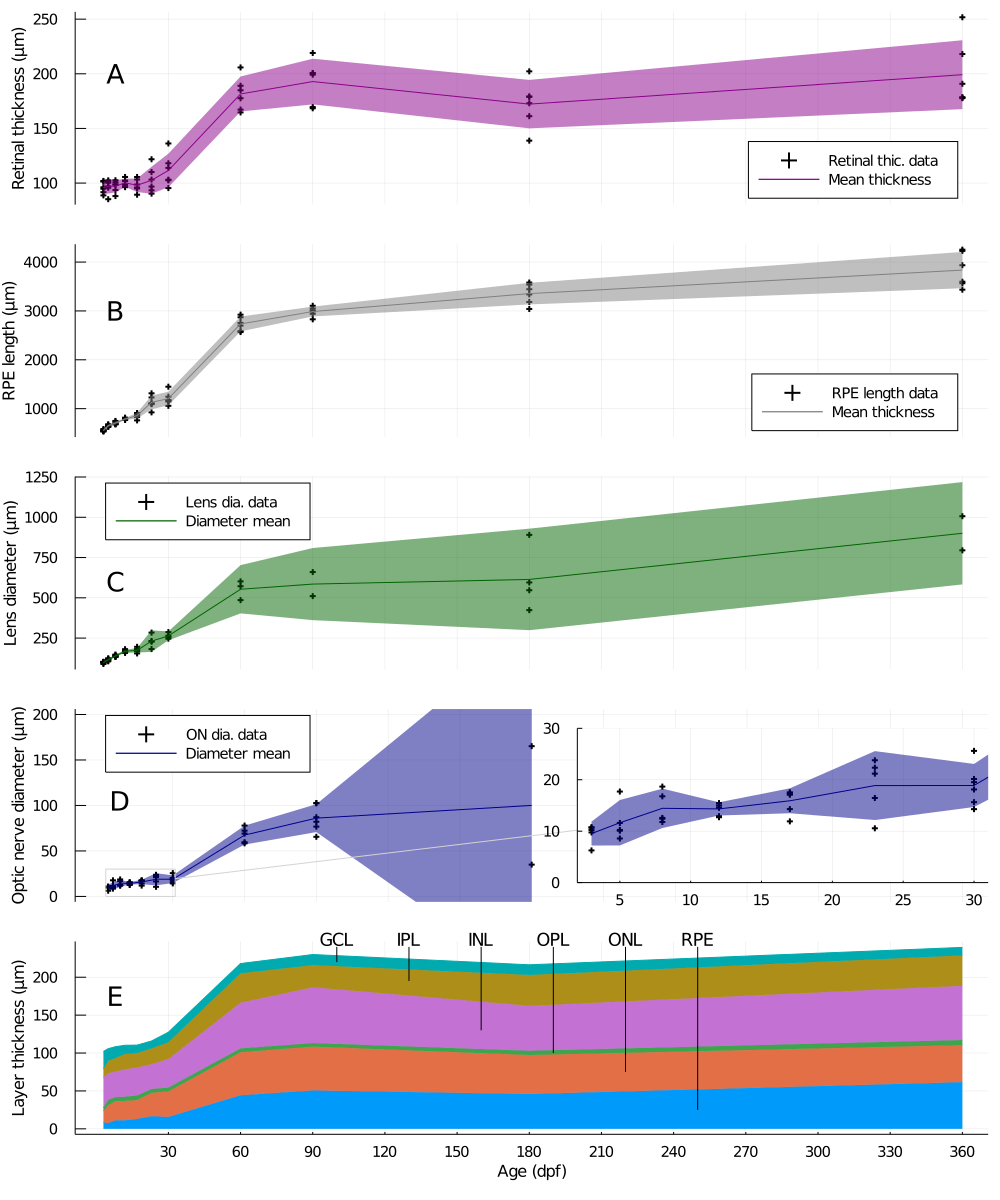
\includegraphics[width=1.\textwidth]{cmz/morphology.png}}    
    \caption{{\bf Overview of \textit{D. rerio} retinal parameters during morphogenesis}}
    All estimates are presented as the marginal posterior distribution of the mean, from uninformative priors, with 95\% credibility intervals.
    Panel A: Thickness of the retina, measured in its center.
    Panel B: Length of the retinal pigmented epithelium, measured from one side of the lens to the other.
    Panel C: Diameter of the lens.
    Panel D: Diameter of the optic nerve, measured in its center.
    Panel E: total thickness of the retina, divided by the thicknesses of the layers that compose it. GCL: Ganglion cell layer. IPL: Inner plexiform layer. INL: Inner nuclear layer. OPL: Outer plexiform layer. ONL: Outer nuclear layers. RPE: Retinal pigmented epithelium.

    Methods in \autoref{ssec:CMZretmeas}. Code in \autoref{ssec:a10morphology}.
    \label{morphology}
\end{figure}

\begin{figure}[!h]
    \makebox[\textwidth][c]{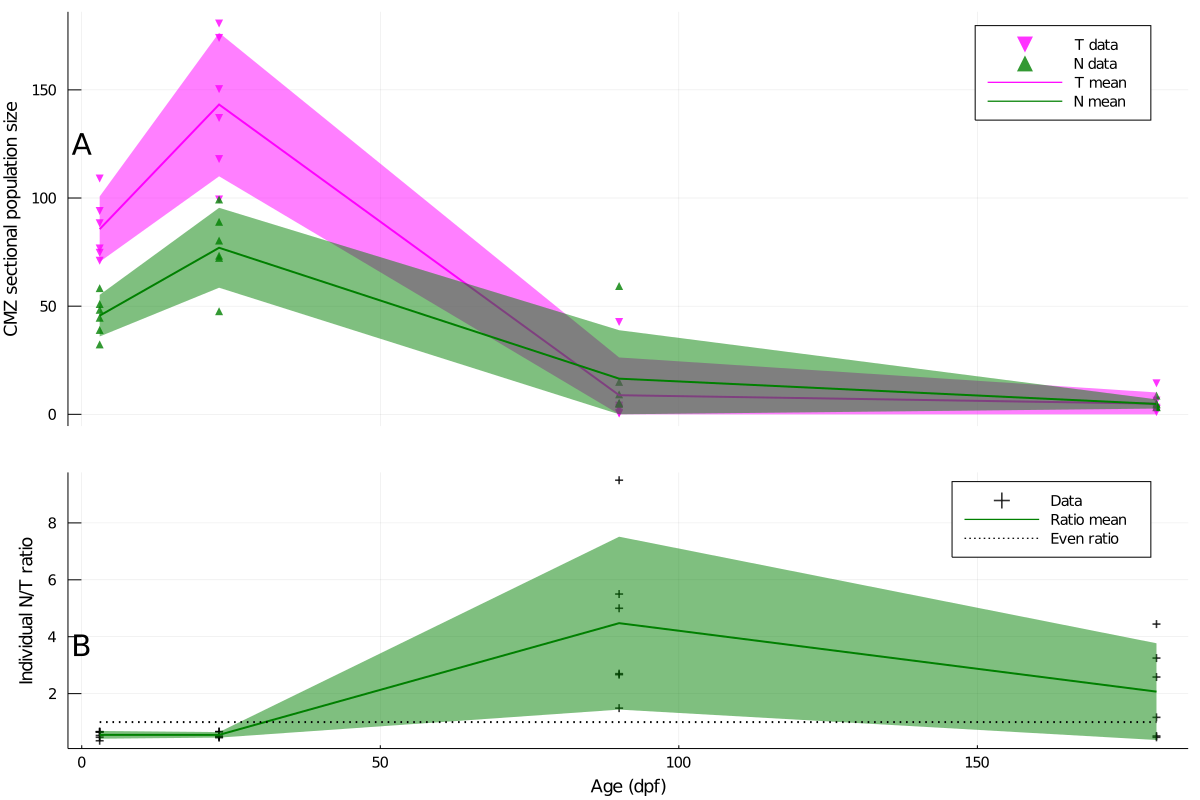
\includegraphics[width=1.2\textwidth]{cmz/NTontology.png}}    
    \caption{{\bf Developmental progression of naso-temporal population asymmetry in the CMZ.}}
    Marginal posterior distribution of mean nasal (N) and temporal (T) population size in 14$\mu$m transverse cryosections (panel A) or intra-individual N/T count asymmetry ratio (panel B), $\pm 95\%$ credible interval, n=6 animals per age. Data points represent mean counts from three central sections of an experimental animal's eye.
    Code in \autoref{ssec:a20dvratio}.
    \label{NTontology}
\end{figure}

\begin{figure}[!h]
    \makebox[\textwidth][c]{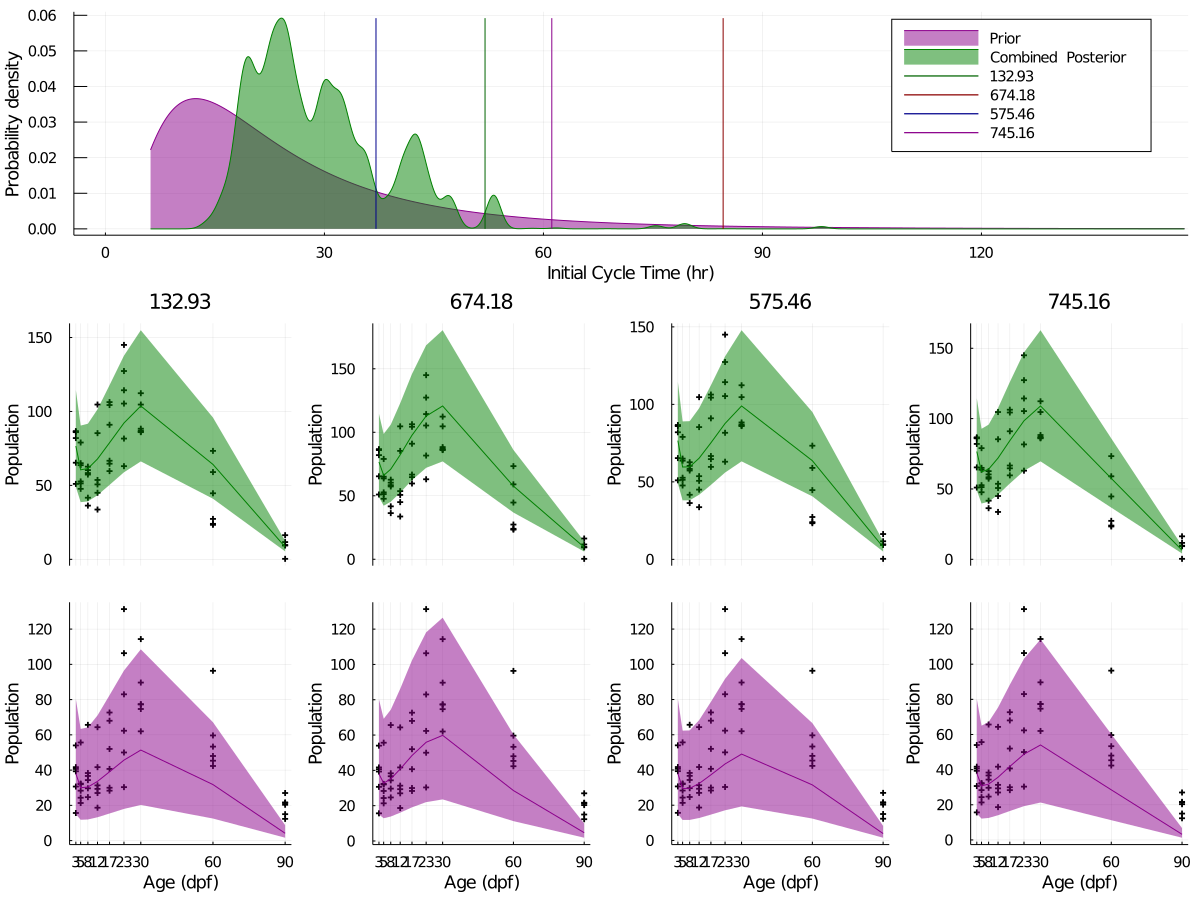
\includegraphics[width=1.\textwidth]{cmz/polymodality.png}}    
    \caption{{\bf Polymodality of CMZ model MAP estimates}}
    Four of the six most likely models found in the MAP sample of the combined decay slice model presented in \autoref{decaymarginals}, located on the marginal distribution of initial cycle time (top panel), and with model output displayed in bottom panels. Note that very different initial CT values produce comparable explanations of the data. Code in \autoref{ssec:a10decayslicediagnostic}.
    \label{polymodality}
\end{figure}

\begin{figure}[!h]
    \makebox[\textwidth][c]{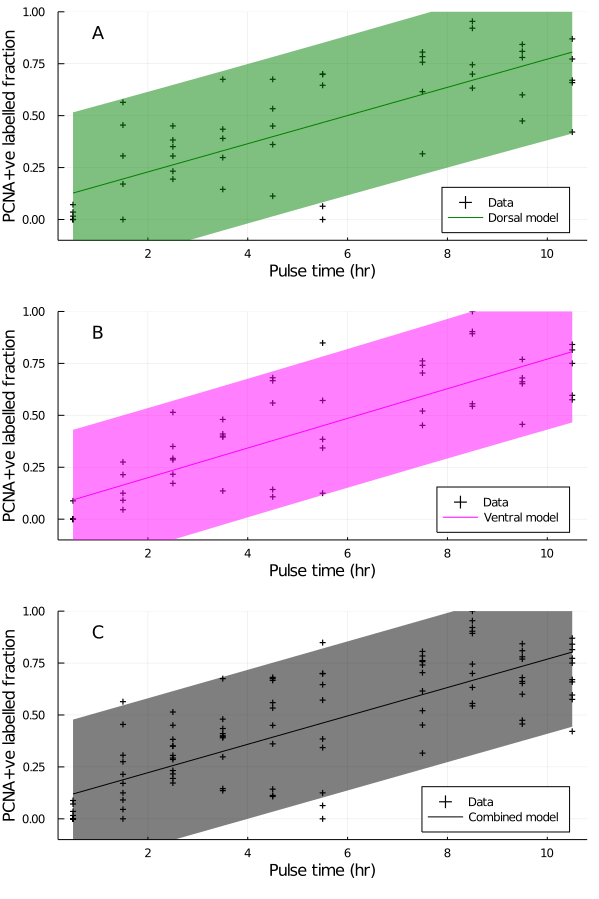
\includegraphics[width=.7\textwidth]{cmz/3ddvlinreg.png}}    
    \caption{{\bf Linear regressions performed on cumulative labelling data from dorsal, ventral, and combined CMZ sectional populations}}
    \label{cumEdUlinreg}
\end{figure}

\begin{figure}[!h]
    \makebox[\textwidth][c]{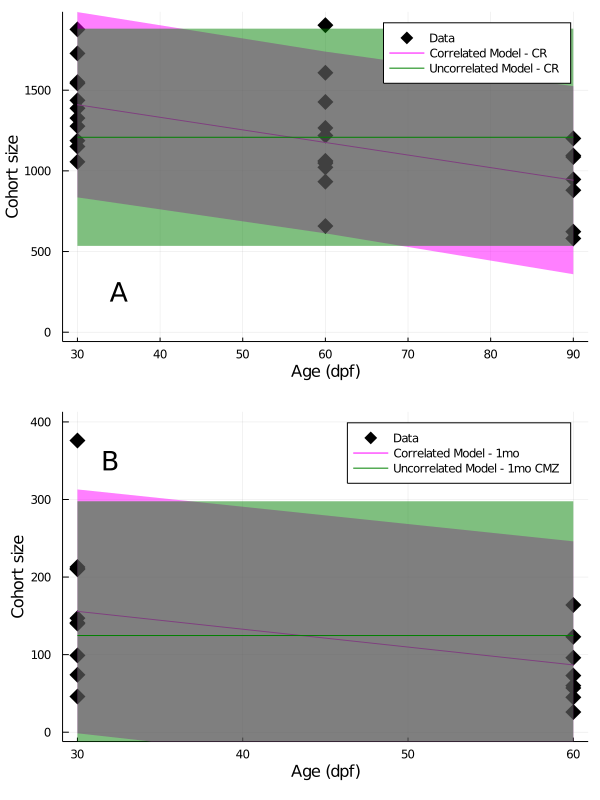
\includegraphics[width=.7\textwidth]{cmz/a27linreg.png}}    
    \caption{{\bf Linear regressions of temporally correlated and uncorrelated models of central retinal and 30dpf CMZ-contributed cohorts}}
    \label{a27linreg}
\end{figure}

\begin{figure}[!h]
    \makebox[\textwidth][c]{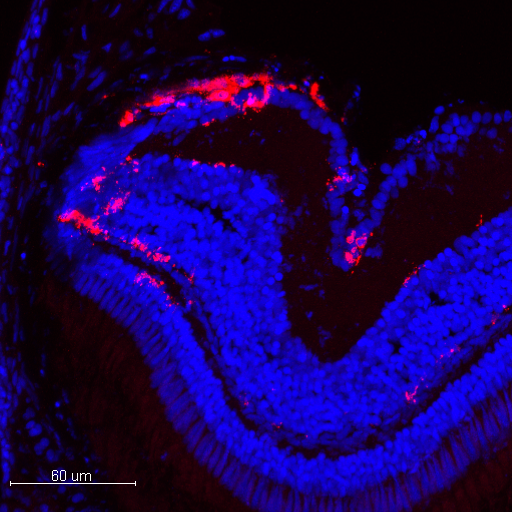
\includegraphics[width=.6\textwidth]{cmz/4C4 distribution.png}}    
    \caption{{\bf 4C4+ microglia are associated with the CMZ}}
    Representative maximum intensity projection from confocal micrographs of 14\si{\micro\metre} coronal cryosections through 90dpf zebrafish eyes.
    
    Blue: Hoechst 33258 nuclear counterstain. Red: Microglia labelled with 4C4 antibody. Note extensive presence of 4C4+ microglia around the peripheral CMZ.
    \label{4C4micrograph}
\end{figure}

\FloatBarrier

\section{Supplementary Tables}
\FloatBarrier

\begin{table}[!ht]
    \caption{{\bf Evidence for Normal vs. Log-Normal models of layer and lineage contribution}}
    \begin{tabular}{|l|l|l|l|l|l|l|} 
        \hline
        {\bf Layer} & {\bf Marker} & {\bf Cell type} & {\bf $\mathcal{N}$ logZ} & {\bf Log-$\mathcal{N}$ logZ} & {\bf logZR} & {\bf $\sigma$ sign.}\\ \hline \hline
        GCL & Cohort & All GCL cells &  -65.52 ± 0.66 & {\bf -30.96 ± 1.0} & 34.6 ± 1.2 & 28.9\\ \hline
        GCL & Isl2b & RGC & -36.64 ± 0.54 & {\bf -23.76 ± 0.59} & 12.88 ± 0.79 & 16.2\\ \hline
        GCL & Pax6 & Displaced am. & {\bf -40.08 ± 0.71} & -40.28 ± 0.46 & -0.19 ± 0.85 & 0.2\\ \hline
        GCL & Isl2b/Pax6 & RGC subtype & -22.09 ± 0.39 & {\bf -16.82 ± 0.83} & 5.27 ± 0.92 & 5.8\\ \hline \hline
        INL & Cohort & All INL cells & {\bf -52.65 ± 0.66} & -120.1 ± 1.4 & -67.5 ± 1.5 & 44.2\\ \hline
        INL & Pax6 & Amacrine cell & -23.09 ± 0.39 & {\bf -9.14 ± 0.46} & 13.95 ± 0.61 & 23.0\\ \hline
        INL & PKC$\beta$ & Bipolar cell & -21.59 ± 0.34 & {\bf 2.81 ± 0.54} & 24.4 ± 0.64 & 38.0\\ \hline
        INL & GS & M\"{u}ller glia & -21.45 ± 0.32 & {\bf 10.18 ± 0.6} & 31.63 ± 0.68 & 46.4\\ \hline
        INL & HM & Horizontal cell & -22.52 ± 0.36 & {\bf 3.02 ± 0.6} & 25.55 ± 0.7 & 36.5\\ \hline \hline
        ONL & Cohort & All ONL cells &{\bf -63.19 ± 0.7} & -81.6 ± 1.3 & -18.5 ± 1.5 & 12.3\\ \hline
        ONL & Zpr1 & Double cones &  {\bf -31.63 ± 0.6} & -26.29 ± 0.6 & 5.34 ± 0.85 & 6.3\\ \hline
    \end{tabular}
    \begin{flushleft}logZ: logarithm of p(D), the marginal likelihood of the data, or model evidence.  Largest evidence values bolded. logZR: evidence ratio; positive values in favour of Log-$\mathcal{N}$ model.
    \end{flushleft}
    \label{lineage_nlnev}
\end{table}

\begin{table}[!ht]
    \caption{{\bf Evidence for combined vs. separate models of layer and lineage contribution across the dorso-ventral axis}}
    \begin{tabular}{|l|l|l|l|l|l|l|} 
        \hline
        {\bf Layer} & {\bf Marker} & {\bf Cell type} & {\bf Combined D-V logZ} & {\bf Split D-V logZ} & {\bf logZR} & {\bf $\sigma$ sign.}\\ \hline \hline
        GCL & Cohort & All GCL cells & {\bf -53.473 ± 0.055} & -184.34 ± 0.13 & 130.86 ± 0.14 & 911.5\\ \hline \hline
        GCL & Isl2b & RGC & {\bf -54.58 ± 0.9} & -67.72 ± 0.94 & 13.1 ± 1.3 & 10.1\\ \hline
        GCL & Pax6 & Displaced am. & {\bf -31.09 ± 0.12} & -46.41 ± 0.3 & 15.32 ± 0.33 & 46.9\\ \hline
        GCL & Isl2b/Pax6 & RGC subtype & {\bf -43.76 ± 0.76} & -109.0 ± 1.3 & 65.3 ± 1.5 & 43.3\\ \hline \hline
        INL & Cohort & All INL cells & {\bf -131.4 ± 1.4} & -184.4 ± 1.6 & 52.9 ± 2.1 & 25.0\\ \hline \hline
        INL & Pax6 & Amacrine cell & {\bf -15.8 ± 0.024} & -52.42 ± 0.69 & 36.62 ± 0.69 & 53.3\\ \hline
        INL & PKC$\beta$ & Bipolar cell & {\bf -3.86 ± 0.2} & -19.81 ± 0.23 & 15.96 ± 0.31 & 51.9\\ \hline
        INL & GS & M\"{u}ller glia & {\bf 15.78 ± 0.25} & 28.03 ± 0.41 & -12.24 ± 0.48 & -25.6\\ \hline
        INL & HM & Horizontal cell & {\bf 10.79 ± 0.41} & -3.65 ± 0.19 & 14.45 ± 0.45 & 32.2\\ \hline \hline
        ONL & Cohort & All ONL cells & {\bf -79.87 ± 0.97} & -158.2 ± 1.3 & 78.3 ± 1.6 & 48.5\\ \hline \hline
        ONL & Zpr1 & Double cones & {\bf -54.66 ± 0.92} & -64.27 ± 0.87 & 9.6 ± 1.3 & 7.6\\ \hline
    \end{tabular}
\begin{flushleft}logZ: logarithm of p(D), the marginal likelihood of the data, or model evidence.  Largest evidence values bolded. logZR: evidence ratio; positive values in favour of combined model.
\end{flushleft}
\label{lineage_dvev}
\end{table}

\begin{table}[!ht]
    \begin{tabular}{|l|l|l|l|l|l|l|} 
        \hline
        {\bf Layer} & {\bf Marker} & {\bf Cell type} & {\bf $\mathcal{N}$ MLE} & {\bf Log-$\mathcal{N}$ MLE} & {\bf lhR}\\ \hline \hline
        GCL & Cohort & All GCL cells & 54.194 & {\bf 55.835} & 1.642\\ \hline
        GCL & Isl2b & RGC & 14.439 & {\bf 19.106} & 4.667\\ \hline
        GCL & Pax6 & Displaced am. &  8.287 & {\bf 11.158} & 2.871\\ \hline
        GCL & Isl2b/Pax6 & RGC subtype & 20.292 & {\bf 28.139} & 7.847\\ \hline
        INL & Cohort & All INL cells & 44.942 & {\bf 45.179} & 0.237\\ \hline
        INL & Pax6 & Amacrine cell & {\bf 23.808} & 23.178 & -0.63\\ \hline
        INL & PKC$\beta$ & Bipolar cell & {\bf 27.243} & 26.119 & -1.124\\ \hline
        INL & GS & M\"{u}ller glia & 30.847 & {\bf 31.818} & 0.97\\ \hline
        INL & HM & Horizontal cell & 27.65 & {\bf 29.431} & 1.78\\ \hline
        ONL & Cohort & All ONL cells & 41.488 & {\bf 43.195} & 1.706\\ \hline
        ONL & Zpr1 & Double cones & 13.256 & {\bf 18.483} & 5.227\\ \hline
    \end{tabular}
   
    \begin{flushleft}logZ: logarithm of p(D), the marginal likelihood of the data, or model evidence.  Largest evidence values bolded. logZR: evidence ratio; positive values in favour of stable model.
    \end{flushleft}
    \label{lineage_lhratio}
\end{table}


